Gibt es einen regulären Ausdruck, mit dem sich die Sprache
\[
L=\{w\in\Sigma^*\;|\; |w|_{\texttt{a}} = |w|_{\texttt{b}}^2\}
\]
über dem Alphabet $\Sigma=\{\texttt{a},\texttt{b}\}$
beschreiben lässt?

\thema{Pumping Lemma für reguläre Sprachen}
\thema{regulär}

\begin{loesung}
Wir beweisen mit dem Pumping Lemma für reguläre Sprachen, dass $L$
nicht regulär sein kann und damit auch nicht mit einem reglären Ausdruck
beschrieben werden kann.
\begin{enumerate}
\item Annahme: $L$ ist regulär.
\item Nach dem Pumping Lemma gibt es die Pumping Length $N$.
\item Sei $l$ die kleinste Zahl, für die $l^2>N$ ist. 
Man kann sie zum Beispiel finden, indem man $\sqrt{N}$ aufrundet.
Wir wählen das Wort
\[
w
=
\texttt{a}^{l^2}\texttt{b}^l
\in
L.
\]
\begin{center}
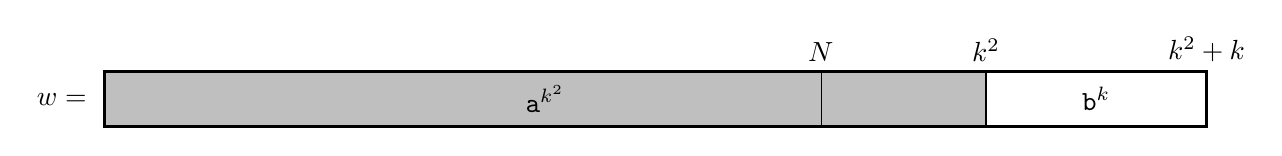
\begin{tikzpicture}[>=latex, scale=0.7]
\node at (0,0.5) [left] {$w=\mathstrut$};
\fill[gray!50] (0,0)--(16,0)--(16,1)--(0,1)--cycle;
\draw[line width=1pt] (0,0)--(20,0)--(20,1)--(0,1)--cycle;
\draw[line width=1pt] (16,0)--(16,1);
\draw[line width=0.1pt] (13,0)--(13,1);
\node at (13,1) [above] {$N$};
\node at (16,1) [above] {$k^2$};
\node at (20,1) [above] {$k^2+k$};
\node at (8,0.5) {$\texttt{a}^{k^2}$};
\node at (18,0.5) {$\texttt{b}^k$};
\end{tikzpicture}
\end{center}
Wegen $|w|_{\texttt{a}} = k^2 = |w|_{\texttt{b}}$ ist $w\in L$.
\item
Wegen $|w|=k^2+k>k^2>N$ ist das Wort lang genug, dass das Pumping Lemma
darauf anwendbar ist.
Das Wort $w$ lässt sich zerlegen in drei Teile
$w={\color{green}x}{\color{red}y}{\color{blue}z}$ mit der
Eigenschaft, dass $xy^kz\in L$ für alle $k\ge 0$:
\begin{center}
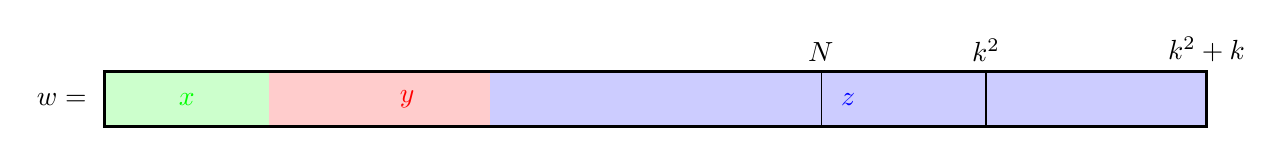
\begin{tikzpicture}[>=latex, scale=0.7]
\fill[color=green!20] (0,0)--(3,0)--(3,1)--(0,1)--cycle;
\fill[color=red!20] (3,0)--(7,0)--(7,1)--(3,1)--cycle;
\fill[color=blue!20] (7,0)--(20,0)--(20,1)--(7,1)--cycle;
\node at (0,0.5) [left] {$w=\mathstrut$};
\draw[line width=1pt] (0,0)--(20,0)--(20,1)--(0,1)--cycle;
\draw[line width=1pt] (16,0)--(16,1);
\draw[line width=0.1pt] (13,0)--(13,1);
\node at (13,1) [above] {$N$};
\node at (16,1) [above] {$k^2$};
\node at (20,1) [above] {$k^2+k$};
\node[color=green] at (1.5,0.5) {$x$};
\node[color=red] at (5.5,0.5) {$y$};
\node[color=blue] at (13.5,0.5) {$z$};
\end{tikzpicture}
\end{center}
\item
Beim Pumpen des Teils $y$ nimmt die Anzahl der Zeichen $\texttt{a}$ 
im Wort zu, ohne dass die Anzahl der Zeichen $\texttt{b}$ verändert wird.
Damit können die gepumpten Wörter nicht in $L$ sein.
\item Diese Widerspruch zeigt, dass $L$ nicht regulär sein kann.
\qedhere
\end{enumerate}
\end{loesung}

\begin{bewertung} 1 Punkt für jeden Schritt des Beweises mit dem
Pumping Lemma:
Annahme ({\bf PL}) 1 Punkt,
Pumping Length ({\bf N}) 1 Punkt,
Beispielwort ({\bf W}) 1 Punkt,
Aufteilung ({\bf A}) 1 Punkt,
Widerspruch beim Pumpen ({\bf P}) 1 Punkt,
Schlussfolgerung ({\bf S}) 1 Punkt.
\end{bewertung}
